\documentclass[11pt,oneside]{book}

\usepackage[a4paper]{geometry}

\linespread{1.2} % Line spacing

\setlength\parindent{0pt} % Uncomment to remove all indentation from paragraphs
\setlength{\parskip}{8pt}

\usepackage[utf8]{inputenc}

\usepackage{lipsum}

\usepackage{amsmath,amssymb,amsthm}
\theoremstyle{plain}
\newtheorem{theorem}{Theorem}[section]
\newtheorem{corollary}{Corollary}[theorem]
\newtheorem{proposition}[theorem]{Proposition}
\newtheorem{lemma}[theorem]{Lemma}

\theoremstyle{definition}
\newtheorem{definition}{Definition}[section]

\theoremstyle{remark}
\newtheorem*{remark}{Remark}

\usepackage{algpseudocode}
\usepackage{algorithm}
\usepackage{listings}
\usepackage{tikz}

\usepackage{subcaption} 
\usepackage{float}
\usepackage{wrapfig}
\usepackage{graphicx}
\graphicspath{{../figures/}}

\usepackage{multirow}
\usepackage{booktabs}
\usepackage{array}

\usepackage{dsfont}
\usepackage{epstopdf}
\usepackage{siunitx}
\usepackage{todonotes}

\usepackage[numbers, sort]{natbib}
\bibliographystyle{plainnat}

\usepackage[nottoc]{tocbibind}

\usepackage{makeidx}
\makeindex

\usepackage{url}

\usepackage{hyperref}
\hypersetup{
    colorlinks,
    citecolor=black,
    filecolor=black,
    linkcolor=black,
    urlcolor=black
}

\usepackage{cleveref}
\usepackage{microtype}

\begin{document}

%----------------------------------------------------------------------------------------
%	TITLE PAGE
%----------------------------------------------------------------------------------------

\begin{titlepage}

\newcommand{\HRule}{\rule{\linewidth}{0.5mm}} % Defines a new command for the horizontal lines, change thickness here

\center % Center everything on the page

\textsc{\Large The University of New South Wales}\\[0.2cm]
\textsc{\large School of Computer Science and Engineering}\\[1.5cm] % Name of your university/college

\textsc{\large Thesis Report - Part A}\\[0.5cm] % Major heading such as course name
\textsc{BSc Computer Science (Honours)}\\[0.5cm] % Minor heading such as course title

\HRule \\[0.4cm]
{ \LARGE \bfseries The Chromatic Derivatives and its Applications }\\[0.4cm] % Title of your document
\HRule \\[1.5cm]

\begin{minipage}[t]{0.4\textwidth}
\begin{flushleft} \large
\emph{Author:}\\
Louis \textsc{Tiao} % Your name
\end{flushleft}
\end{minipage}
~
\begin{minipage}[t]{0.5\textwidth}
\begin{flushright} \large
\emph{Supervisor:} \\
Dr. Aleksandar \textsc{Ignjatovi\'{c}} % Supervisor's Name
\\[0.5cm]
\emph{Assessor:} \\
Dr. Alan \textsc{Blair} % Assessor's Name
\end{flushright}
\end{minipage}\\[4cm]

{\large \today}\\[3cm] % Date, change the \today to a set date if you want to be precise

%\includegraphics{Logo}\\[1cm] % Include a department/university logo - this will require the graphicx package

\vfill % Fill the rest of the page with whitespace

\end{titlepage}

\newpage 

\thispagestyle{plain}

\topskip0pt
\vspace*{\stretch{1}}
\begin{center}
{\large
  \emph{Dedicated to memory of my beloved grandfather, \\ 
  Hai-Xiang Tiao (1918--2014).}
}  
\end{center}
\vspace*{\stretch{3}}

% \par\vspace*{.35\textheight}
% {\centering \dedicatory{Dedicated to memory of my grandfather, 1918--2014.}\par}

\newpage

%----------------------------------------------------------------------------------------
%	TABLE OF CONTENTS
%----------------------------------------------------------------------------------------

\tableofcontents % Include a table of contents

\newpage

%----------------------------------------------------------------------------------------
%	INTRODUCTION
%----------------------------------------------------------------------------------------

\chapter{Introduction} \label{intro} % Major section

It is no overstatement that the Nyquist-Shannon sampling theorem
 is indispensable to the fields of communication and signal processing. It 
allows us to convert continuous real-world analog signals into discrete signals, 
represented as a sequence a numbers, to then be processed and manipulated digitally on a 
computer - it makes digital signal processing possible, both in theory and in practice.

Let $f$ be a signal of finite energy bandlimited by $B$, i.e. $f$ is a continuous $L^2$ 
function whose Fourier transform has support within $[-B,B]$. We denote the class of
such functions $\mathbf{BL}(B)$. The interpolation (reconstruction) formula complementary to the 
sampling theorem, commonly known as the Whittaker–Shannon interpolation formula, is
given by
\begin{equation} \label{eq:whittaker_shannon}
  f(t) = \sum_{n=-\infty}^{\infty} f(n) \mathrm{sinc}(t-n)
\end{equation}
where $\mathrm{sinc}$ is the (normalized) cardinal sine function, defined by 
$\mathrm{sinc}(x)=\frac{\sin{\pi x}}{\pi x}$ for $x \neq 0$ and $\mathrm{sinc}(0)=1$.

This series expansion in \cref{eq:whittaker_shannon} can be seen as a special case of the 
generalized Fourier series, with the complete orthonormal system of univariate functions 
$\{ \mathrm{sinc}(t-n) \}_{n\in\mathbb{Z}}$ as its basis. Roughly speaking, the interpolation
formula given by \cref{eq:whittaker_shannon} and Fourier series in general are ``global'' in 
the sense that it requires the samples of the signal at integer points of arbitrarily large 
absolute value, i.e. values at points spanning a large part of its domain. Additionally, 
the truncation error of Fourier series is distributed along the domain of the function.

On the other hand, consider a signal $f \in \mathbf{BL}(\pi)$, which is also an analytic 
function. Its Taylor series expansion about point $t=t_0$ is given by
\begin{equation} \label{eq:taylor}
  f(t) = \sum_{n=0}^{\infty} f^{(n)}(t_0) \frac{(t-t_0)^n}{n!}
\end{equation}
We mainly consider the expansion about point $t_0=0$, which is also known as the Maclaurin series.
The Taylor series are said to ``local'' in the sense that values of the $n$th order derivatives 
$f^{(n)}(t_0)$ can be obtains by samples of the signal on an arbitrarily small neighborhood
of $t_0$. It is no surprise then that the truncation error of Taylor series is very small in the 
neighborhood on which it has been computed and grows dramatically as we move away from this neighborhood.

In stark contrast to the Shannon-Whittaker interpolation, the Taylors series, though 
instrumental in mathematical analysis, finds relatively limited use in digital signal 
processing, due to its multitude of shortcomings. We give a brief overview of these problems
now, and extend our discussion in \cref{freq_response}.

\begin{enumerate}
  \item numerical evaluation of derivatives, let alone those of higher orders are
    highly sensitive to noise.
  \item the Taylor series expansion of a signal $f \in \mathbf{BL}(\pi)$ does not
    converge uniformly on $\mathbb{R}$.
  \item as mentioned already, truncation error of Taylor series accumulates quite rapidly.
  \item the Shannon-Whittaker interpolation of signal $f \in \mathbf{BL}(\pi)$ converges
    to $f$ in $\mathbf{BL}(\pi)$ while the truncations (approximation by finite sum) of the
    Taylor series expansion do not even belong to $\mathbf{BL}(\pi)$.
  \item For any input signal $f \in \mathbf{BL}(\pi)$ to a continuous, linear, time-invariant 
    system $L$, its output can be characterized entirely by samples of the signal 
    and the impulse response of the system, $L[\mathrm{sinc}]$. More concisely,
    \begin{equation}
      L[f](t) = \sum_{n=-\infty}^{\infty} f(n) L[\mathrm{sinc}](t-n)
    \end{equation}
    Nothing resembling this holds for the Taylor series expansions.
\end{enumerate}

In light of these problems, it is no wonder we see little application of Taylor series
in digital signal processing. This is a pity, because there are a number of (albeit unusual) 
problems in signal processing that require processing and analyzing signals on an extremely
local and almost microscopic level. Examples include designing signal processors that exploit 
the predictive properties of the signal, methods for image reconstruction problems that 
specifically depend on information from local regions of the images rather than from the 
image as a whole, and adaptive filtering applications.

Since Taylor series cannot readily be applied to these problems, we must reconcile 
the local properties of the Taylor series with the ideal features of the Fourier 
series that make it so crucial to digital signal processing.

To alleviate some of the problems that render Taylor series ineffective for signal processing, 
the \emph{chromatic derivatives} were introduced by Dr.~Ignjatovi\'{c} in 2000 \cite{ignjatovic2000signal}. 
Naturally, the
theory emerged in the conception of a novel switching amplifier with the ability anticipate
(predict) future signal values by exploiting the local signal behavior.

The \emph{chromatic expansions}, complementary to the chromatic derivatives, were later introduced \cite{ignjatovic2001method} 
and several applications and novel techniques that harness the theory of chromatic derivatives
were subsequently proposed. Some of these include the design of communication channel
equalizers \cite{herron2001towards}, digital transceivers, image compression methods \cite{cushman2001method}.

The theory has since been generalized and extended to systems corresponding to several classical 
families of orthogonal polynomials \cite{Cushman2001,Herron2001} and cast in to the conventional 
signal processing framework \cite{Vaidyanathan2001,Narasimha2002}. 
More recently, the chromatic derivatives and expansions were generalized to 
multiple dimensions \cite{Ignjatovic2011a}.

We believe (multidimensional) chromatic derivatives and expansions lends itself naturally
to many applications in important fields such as image processing. The exploration, 
conception and implementation of some these applications will be the subject of this thesis. 

This report is structured as follows. In \cref{cd_def}, we formally define the chromatic 
derivatives, specifically those associated with the Legendre polynomials. For a concise and more 
generalized exposition of chromatic derivatives, please consult \cite{Ignjatovic2009}, which also 
forms the basis for this present report. Continuing in \cref{cd_expansion}, we discuss some of its 
properties, and contrast chromatic expansions with Taylor/Fourier series expansions with some 
examples. In \cref{image_applications}, we outline some of the image processing problems we intend 
to tackle and give a brief literature review of the conventional methods used to solve these problems. 
Finally, in \cref{proposal} we propose our approach to solving these problems with the machinery of 
multidimensional chromatic derivatives, and roughly outline the plan for carrying out our approach.

\newpage

\chapter{Background}

\section{Preliminaries}

The \emph{Legendre functions} are solutions to the \emph{Legendre differential 
equation}, which is the second-order ordinary differential equation

\begin{equation} \label{eq:legendre_de}
\frac{d}{dx}\left[(1-x^2)\frac{d}{dx}L_n(x)\right]+n(n+1)L_n(x)=0
\end{equation}

The \emph{Legendre polynomials}, also known as \emph{Legendre functions of the 
first kind}, satisfy the following recurrence relation:
\begin{align}
L_0(x)     &= 1 \\
L_1(x)     &= x \\
L_{n+1}(x) &= \frac{2n+1}{n+1} x L_n(x) - \frac{n}{n+1} L_{n-1}(x)
\end{align}
The Legendre polynomials are orthogonal (and complete) over the closed interval 
$[-1, 1]$
\begin{equation*}
  \frac{1}{2}\int_{-1}^{1} L_n(x)L_m(x) dx = \frac{1}{2n+1} \delta_{mn}
\end{equation*}
where $\delta_{ij}$ is the Kronecker delta:
\begin{equation}
  \delta_{ij} =
    \begin{cases}
     0       & \text{for } i \neq j, \\
     1       & \text{for } i = j.
    \end{cases}
\end{equation}
We can easily normalize and scale to obtain Legendre polynomials that are
orthogonal (and complete) over the closed interval $[-\pi,\pi]$
\begin{equation}
  P_n^L(x) = \sqrt{2n+1}L_n\left(\frac{x}{\pi}\right)
\end{equation}
so that 
\begin{equation*}
\frac{1}{2\pi} \int_{-\pi}^{\pi} P_n^L(x)P_m^L(x) dx = \delta_{mn}
\end{equation*}
Likewise, it satisfies the recurrence relation
\begin{align}
P_0^L(x)     &= 1 \\
P_1^L(x)     &= \frac{\sqrt{3}}{\pi} x \\
P_{n+1}^L(x) &= \frac{\sqrt{4(n+1)^2-1}}{(n+1) \pi} x P_n^L(x) - \frac{n\sqrt{4(n+1)^2-1}}{(n+1)\sqrt{4n^2-1}} P_{n-1}^L(x)
\end{align}
More concisely, we can define this as
\begin{align}
  P_{n+1}^L(x) = \frac{1}{\gamma_n} x P_n(x) - \frac{\gamma_{n-1}}{\gamma_n} P_{n-1}(x)
\end{align}
with $P_{-1}(x)=0, P_0(x)=1$, and
\begin{equation}
  \gamma_n = \frac{(n+1) \pi}{\sqrt{4(n+1)^2-1}}
\end{equation}
with $\gamma_{-1} = 1$.

\section{Chromatic derivatives}

\subsubsection{Definition} \label{cd_def}

The chromatic derivatives associated with Legendre polynomials are defined as
\begin{equation}
  \mathcal{K}_t^n = (-i)^n P_n^L \left (i \frac{d}{dt} \right )
\end{equation} 
When applied to univariate functions, there should be no ambiguity as to
which variable we are differentiating with respect to, so we can use Heaviside's
notation to denote the differential operator, i.e. $\mathcal{D} = \mathcal{D}_t 
= \frac{d}{dt}$. 

So now we have
\begin{equation}
  \mathcal{K}^n = (-i)^n P_n^L \left (i \mathcal{D} \right )
\end{equation}
and this of course satisfies the recurrence relation
\begin{equation}
  \mathcal{K}^{n+1} = \frac{1}{\gamma_n} \left ( \mathcal{D} \circ \mathcal{K}^n \right ) 
                        + \frac{\gamma_{n-1}}{\gamma_n} \mathcal{K}^{n-1}
\end{equation}
with $\mathcal{K}^{-1} = 0, \mathcal{K}^0 = \mathds{1}$ where $\mathds{1}$ is 
the identity operator and $\gamma_n$ are as defined as before. Note that 
$\mathcal{K}^{-1}$ signifies the constant 0 operator.

Now, it is easy to see that
\begin{equation}
  \mathcal{K}_t^n[e^{i\omega t}] = i^n P_n^L(\omega) e^{i\omega t}
\end{equation}
since the polynomials $P_n^L(x)$ contains only variables with powers of the same
parity as that of $n$, and the operators $\mathcal{K}_t^n$ only have real coefficients.

Let $x(t) \in \mathbf{BL}(\pi)$. We now have,
\begin{align*}
  \mathcal{K}_t^n[x(t)]
    &= \mathcal{K}_t^n[\mathcal{F}^{-1}[X(\omega)]] \\
    &= \mathcal{K}_t^n \left [ \frac{1}{2 \pi} \int_{-\infty}^{\infty} X(\omega) e^{i \omega t} d\omega \right ] \\
    &= \frac{1}{2 \pi} \int_{-\infty}^{\infty} X(\omega) \mathcal{K}_t^n[e^{i \omega t}] d\omega \\
    &= \frac{1}{2 \pi} \int_{-\infty}^{\infty} i^n P_n^L(\omega) X(\omega) e^{i\omega t} d\omega \\
    &= \frac{1}{2 \pi} \int_{-\pi}^{\pi} i^n P_n^L(\omega) X(\omega) e^{i\omega t} d\omega \\
\end{align*}

\begin{remark}
We denote the Fourier transform and its inverse respectively as 
\begin{align}
  X(\omega) &= \mathcal{F}[x(t)] = \int_{-\infty}^{\infty} x(t) e^{-i \omega t} dt \\
  x(t)      &= \mathcal{F}^{-1}[X(\omega)] = \frac{1}{2 \pi} \int_{-\infty}^{\infty} X(\omega) e^{i \omega t} d\omega
\end{align}
\end{remark}

\subsubsection{Frequency response} \label{freq_response}

Systems (operators) can have a variety of effects on input signals of different frequencies, 
e.g. they may amplify certain frequency components while attenuating others. The \emph{frequency 
response} of a system is the way the system output relates to the system input signals for 
different frequencies in the frequency domain. More precisely, consider the input signal $X(\omega)$
in the frequency domain. Denote the system output as $Y(\omega)$. The frequency response $H(\omega)$ 
satisfies the relationship
\begin{equation}
  Y(\omega) = H(\omega) X(\omega)
\end{equation}
and is therefore given by
\begin{equation}
  H(\omega) = \frac{Y(\omega)}{X(\omega)}
\end{equation}
Let us now contrast the frequency response of the normalized $n$th order differential 
operator $\frac{1}{\pi^n} \frac{d^n}{dt^n} = \frac{1}{\pi^n} \mathcal{D}_t^n$ with that 
of the chromatic derivative operator $\mathcal{K}_t^n$.

Let $x(t) \in \mathbf{BL}(\pi)$,
\begin{align*}
  y(t) &= \frac{1}{\pi^n} \mathcal{D}_t^n[x(t)] \\
       &= \frac{1}{\pi^n} \mathcal{D}_t^n[\mathcal{F}^{-1}[X(\omega)]] \\
       &= \frac{1}{\pi^n} \mathcal{D}_t^n \left [ \frac{1}{2 \pi} \int_{-\infty}^{\infty} X(\omega) e^{i \omega t} d\omega \right ] \\
       &= \frac{1}{2 \pi} \int_{-\infty}^{\infty} X(\omega) \frac{1}{\pi^n} \mathcal{D}_t^n[e^{i \omega t}] d\omega \\
       &= \frac{1}{2 \pi} \int_{-\infty}^{\infty} i^n \left(\frac{\omega}{\pi}\right)^n X(\omega) e^{i\omega t} d\omega \\
       &= \frac{1}{2 \pi} \int_{-\infty}^{\infty} Y(\omega) e^{i\omega t} d\omega
\end{align*}

So now we have 
\begin{equation*}
  Y(\omega) = i^n \left(\frac{\omega}{\pi}\right)^n X(\omega)
\end{equation*}
and therefore
\begin{equation*}
  H(\omega) = \frac{Y(\omega)}{X(\omega)} = \frac{i^n \left(\frac{\omega}{\pi}\right)^n X(\omega)}{X(\omega)} = i^n \left(\frac{\omega}{\pi}\right)^n
\end{equation*}

Since the frequency response is a complex function, we can decompose it further 
into its complex modulus and argument, respectively called the \emph{amplitude response}
and \emph{phase response}. We will look specifically at the amplitude response, which 
represents the system's tendency to amplify or attenuate the signal.

The amplitude response is given by
\begin{equation*}
  |H(\omega)| = \left|i^n \left(\frac{\omega}{\pi}\right)^n\right| 
              = |i^n| \cdot \left|\left(\frac{\omega}{\pi}\right)^n\right| 
              = \frac{1}{\pi^n} |\omega|^n
\end{equation*}
and is plotted in \cref{fig:amp_response1} for $n=15, \dotsc, 18$.

Now let us look at the frequency response of the chromatic derivative operator. We first compute 
the output of the system as before
\begin{align*}
  y'(t) &= \mathcal{K}_t^n[x(t)] \\
        &= \frac{1}{2 \pi} \int_{-\infty}^{\infty} i^n P_n^L(\omega) X(\omega) e^{i\omega t} d\omega \\
        &= \frac{1}{2 \pi} \int_{-\infty}^{\infty} Y'(\omega) e^{i\omega t} d\omega
\end{align*}
So we have
\begin{equation*}
  Y'(\omega) = i^n P_n^L(\omega) X(\omega)
\end{equation*}
and therefore
\begin{equation*}
  H'(\omega) = \frac{Y'(\omega)}{X(\omega)} = \frac{i^n P_n^L(\omega) X(\omega)}{X(\omega)} = i^n P_n^L(\omega)
\end{equation*}
The amplitude response is given by
\begin{equation*}
  |H'(\omega)| = |P_n^L(\omega)|
\end{equation*}
and is plotted in \cref{fig:amp_response2} for $n=15, \dotsc, 18$.

\begin{figure}[H]
  \centering
  \caption{Amplitude responses of the differential (left) and chromatic derivative (right) operators for $n=15, \dotsc, 18$.}
  \begin{subfigure}[b]{0.49\textwidth}
    \includegraphics[width=\textwidth]{amplitude_response1.pdf}
    \caption{Amplitude response $H(\omega)$}
    \label{fig:amp_response1}
  \end{subfigure}
  \hfill
  \begin{subfigure}[b]{0.49\textwidth}
    \includegraphics[width=\textwidth]{amplitude_response2.pdf}
    \caption{Amplitude response $H'(\omega)$}
    \label{fig:amp_response2}
  \end{subfigure}
\end{figure}

Just from visually comparing these plots alone, the differences are striking. We see in
\cref{fig:amp_response1} that the frequency response not only attenuates the frequency
components of the signal, it practically obliterates its entire spectrum, save maybe for 
its edges which in practice contains mostly noise anyway. This is the essence of why 
numerical evaluation of higher order derivatives from signal samples makes no practical 
sense.

Fortunately, this does not imply numerical evaluation of higher order derivatives is
inherently unfeasible. Unlike the set of differential operators $\{\mathcal{D}^n\}_
{n\in\mathbb{Z}}$, the set of chromatic derivative operators $\{\mathcal{K}^n\}_
{n\in\mathbb{Z}}$ is an orthogonal basis for the vector space of linear differential 
operators with real coefficients.

A \emph{comb filter} adds a delayed version of a signal to itself, causing constructive 
and destructive interference. From \cref{fig:amp_response2}, we see that the amplitude
response of the chromatic derivative operators form a family of feedforward comb filters
that are well-separated, interleaved, and increasingly refined. Rather than attenuating
frequency components, it encodes and augments the frequency components of the signal
and overall preserves its spectral features.

\subsubsection{Chromatic expansions} \label{cd_expansion}

Let $x(t) \in \mathbf{BL}(\pi)$. We can write its Fourier transform $X(\omega)$ as a 
generalized Fourier series
\begin{equation*}
  X(\omega) = \sum_{n=0}^{\infty} a_n (-i)^n P_n^L(\omega)
\end{equation*}
since we can plug this into the orthogonality relationship of Legendre polynomials to obtain
\begin{align*}
  \int_{-\pi}^{\pi} X(\omega) i^m P_m^L(\omega) d\omega 
    &= \int_{-\pi}^{\pi} \left ( \sum_{n=0}^{\infty} a_n (-i)^n P_n^L(\omega) \right ) i^m P_m^L(\omega) d\omega \\
    &= \sum_{n=0}^{\infty} a_n (-i)^n  i^m \int_{-\pi}^{\pi} P_n^L(\omega) P_m^L(\omega) d\omega \\
    &= 2 \pi \sum_{n=0}^{\infty} a_n (-i)^n  i^m \delta_{mn} \\
    &= 2 \pi a_m
\end{align*}
Therefore, 
\begin{equation*}
  a_m = \frac{1}{2\pi} \int_{-\pi}^{\pi} X(\omega) i^m P_m^L(\omega) d\omega 
      = \mathcal{K}_t^m[x(t)] |_{t=0} = \mathcal{K}^m[x](0)
\end{equation*}
Now we take the inverse Fourier transform
\begin{align*}
  x(t) = \mathcal{F}^{-1}[X(\omega)] 
      &= \frac{1}{2 \pi} \int_{-\infty}^{\infty} X(\omega) e^{i \omega t} d\omega \\
      &= \frac{1}{2 \pi} \int_{-\pi}^{\pi} X(\omega) e^{i \omega t} d\omega \\
      &= \frac{1}{2 \pi} \int_{-\pi}^{\pi} \left ( \sum_{n=0}^{\infty} a_n (-i)^n P_n^L(\omega) \right ) e^{i \omega t} d\omega \\
      &= \sum_{n=0}^{\infty} a_n \left ( \frac{1}{2 \pi} \int_{-\pi}^{\pi} (-i)^n P_n^L(\omega) e^{i \omega t} d\omega \right ) \\
      &= \sum_{n=0}^{\infty} a_n \sqrt{2n+1} j_n(\pi t) \\
      &= \sum_{n=0}^{\infty} \mathcal{K}^m[x](0) \sqrt{2n+1} j_n(\pi t) \\
\end{align*}
where $j_n(\omega) = \sqrt{\frac{\pi}{2\omega}} J_{n+\frac{1}{2}}(\omega)$ are the spherical Bessel functions.

Thus, we arrive at the chromatic expansion associated with Legendre polynomials
\begin{equation}
  f(t) = \sum_{n=0}^{\infty} \mathcal{K}^m[f](0) \sqrt{2n+1} j_n(\pi t)
\end{equation}
More generally, let $f(t)$ be any function analytic on $\mathbb{R}$. Then for all $t\in\mathbb{R}$,
\begin{align}
  f(t) &= \sum_{n=0}^{\infty} K^n[f](u) K_u^n[\mathrm{sinc}(t-u)] \\
       &= \sum_{n=0}^{\infty} (-1)^n K^n[f](u) K^n[\mathrm{sinc}](t-u)
\end{align}

and if $f \in \mathbf{BL}(\pi)$, then the series converges uniformly on $\mathbb{R}$ 
and also in $\mathbf{BL}(\pi)$.

\begin{figure}[H]
  \centering
  \caption{Plot of sinusoidal $\frac{1}{10} \sin \left(\frac{3 \pi  t}{10}\right)+\cos \left(\frac{\pi  t}{5}\right)+\frac{1}{5} \cos \left(\frac{9 \pi  t}{10}\right)$ (red), its Taylor series approximation (blue), Shannon-Whittaker interpolation (green) and chromatic approximation (yellow), all with 21 terms.}
  \begin{subfigure}[b]{0.49\textwidth}
    \includegraphics[width=\textwidth]{interpolation1.pdf}
    \caption{Approximations}
    \label{fig:interpolation1}
  \end{subfigure}
  \hfill
  \begin{subfigure}[b]{0.49\textwidth}
    \includegraphics[width=\textwidth]{interpolation2.pdf}
    \caption{Absolute error}
    \label{fig:interpolation2}
  \end{subfigure}
\end{figure}

As an example, consider the sinusoidal signal $f(t) = \frac{1}{10} \sin \left(\frac{3 \pi  t}{10}\right)+\cos 
\left(\frac{\pi  t}{5}\right)+\frac{1}{5} \cos \left(\frac{9 \pi t}{10}\right)$, which is plotted in \cref{fig:interpolation1} 
in red. The chromatic approximation of order 21 is shown in yellow, while the Taylor series of order 21 and Whittaker-Shannon 
interpolation with 21 terms are shown in blue and green respectively. The same color coding scheme applies to \cref{fig:interpolation2},
which plots the absolute errors of each approximation. Immediately, we see that the truncation error of Taylor series
explodes quite dramatically as we move away from the point of expansion, while the error accumulation of the chromatic
approximation is quite gentle - even comparable to that of the Whittaker-Shannon interpolation.

\subsubsection{Properties} 

To contrast the chromatic derivatives and its expansion with Taylor series expansions,
we consider some of its properties. Compare these with the issues outlined in \cref{intro}. 

\begin{itemize}
  \item The chromatic approximations are bounded on $\mathbb{R}$ and belong to $\mathbf{BL}(\pi)$.
  \item As mentioned already, unlike Taylor series expansions, if $f \in \mathbf{BL}(\pi)$, 
    then the series converges uniformly on $\mathbb{R}$ and also in $\mathbf{BL}(\pi)$.
  \item The above property implies that if $L$ is a filter, then $L$ commutes with the differential
    operators $K^n$. Therefore, for every $f \in \mathbf{BL}(\pi)$,
    \begin{equation}
      L[f](t) = \sum_{n=0}^{\infty} (-1)^n \mathcal{K}^n[f](0) \mathcal{K}^n[L[\mathrm{sinc}]](t)
    \end{equation}
\end{itemize}

Despite the above dissimilarities, the chromatic approximation are local, 
like the Taylor series approximation,  since its coefficients are the values 
of the differential operators $\mathcal{K}^n[f](u)$ at instant $u$.

So we see that chromatic expansions, while local, still possesses the important 
properties that make the Whittaker-Shannon interpolation so essential to 
digital signal processing. These features, coupled with the numerical robustness
(noise tolerance) of chromatic derivatives, makes the chromatic approximations
important and useful for processing and analyzing empirically sampled data, 
and promises applications in digital signal processing and related fields 
such as image processing. 

\section{Image processing applications} \label{image_applications}

We now consider some problems which chromatic derivatives naturally
lends itself to, specifically those in the field of image processing. This
is of course by no means an exhaustive list of problems the chromatic derivatives 
can address but rather the problems we are most interested in solving
as part of this thesis project. 

\subsubsection{Padding for neighborhood operations}

A linear filter is a type of \emph{neighborhood operator} that uses a weighted 
combination of the pixel values in the vicinity of a given pixel to determine 
its final output value.

Denote $f(i, j)$ the original pixel value and let $h(k, l)$ be the 
\emph{convolution matrix} or \emph{kernel}. The \emph{convolution} between 
$f$ and $h$ is given by
\begin{align} \label{eq:linear_filter_convolution}
  g(i, j) = [f \ast h](i, j)  &= \sum_k \sum_l f(i-k, j-l) \cdot h(k, l) \\
                &= \sum_k \sum_l f(k, l) \cdot h(i-k, j-l)  \nonumber
\end{align}

The linear filter is commonly used to create a wide range of effects, 
such as adding  soft blurs, sharpening details, accentuating edges, etc.

Note that the summations defined \cref{eq:linear_filter_convolution} is over
all values of $k$ and $l$. This is because the values of $f$ and $h$ will usually
be 0 for values outside of a defined region. For an image of dimensions, (i.e.
height and width respectively) $M$ and $N$, for all $i<0$ or $i \geq M$ and $j<0$ 
or $j \geq N, f(i,j)=0$. Similarly, if a kernel $h$ is of size $(K, K)$, then for
all $|k|>K$ or $|l|>K, h(k,l)=0$.  

One obvious problem that arises is that the convolution operation requires 
pixel values that are outside the boundaries of the image. By default these
values would be padded by zeros, which basically corresponds to a black frame
surrounding the image. Several alternative approaches are taken, such 
as

\begin{description}
  \item[constant] set all pixel values outside the border to some constant value
  \item[clamp] replicate the edge pixels indefinitely
  \item[wrap] repeat/tile the image indefinitely
  \item[mirror] reflect pixels across image border
  \item[crop] ignore the positions which would require pixel values outside the border,
    effectively cropping the image by $K$ on each side of the image.
\end{description}

Please consult \citet[p.~111-115]{Szeliski2011} for an extended discussion
of linear filters and the various padding modes employed in practice. 

All of these modes can be formulated mathematically 
\cite[see][p.~114-115]{Szeliski2011}. For example, the clamp mode can be expressed 
as follows. Let $\tilde{f}(i, j)$ be \emph{extended} pixel values, defined for all 
$i, j$. We can express it as a function of the original pixel values $f(k, l)$ and the 
dimensions (height, width) of the image $(M, N)$.
\begin{align*}
  \tilde{f}(i, j) &= f(k, l), \\
  k               &= \max(0, \min(M-1, i)), \\
  l               &= \max(0, \min(N-1, j)).
\end{align*}

The alternative method we propose is to essentially ``estimate'' the values $f(i,j)$
for $i<0$ or $i \geq M$ and $j<0$ or $j \geq N$ and effectively extend the image in 
a visually plausible manner. Note that we need only extend the image by as far
as $\lceil \frac{K}{2} \rceil$ pixels beyond the boundaries.

This problem is well-suited to (multidimensional) chromatic derivatives since we
can sample the image and place emphasis on the local boundary sample 
values in order to approximate the values beyond the boundaries. This can be seen as a
special (easier) case of the next problem, so can serve to warm us up and equip
us to tackle the next problem.

\subsubsection{Digital image inpainting}

Inpainting is the process of reconstructing lost or deteriorated portions of an 
image. The overarching objectives are to restore its unity and visual consistency. 
Traditionally, it is practiced by professional conservator-restorators to restore 
and retouch damaged artwork. Nowadays, digitalized methods of inpainting are used on 
digital images for such things as refilling the gaps left from the removal of undesirable
object or artifacts from images, such as blemishes, date stamps, and sometimes even people (see \cref{fig:inpaint_ex}).

Digital techniques for inpainting are widespread and supported by popular photo/graphics 
editing tools. However, to achieve desirable results, digital inpainting remains a mostly manual (and often laborious) process.  

In recent year, methods to completely automate the process of digital image inpainting 
have received considerable research interest, and the methods devised thus
far have demonstrated convincing results. Of course, when we say automate, some level of
user interaction is still required; the user must select the region to be removed. 

\begin{figure}[H]
  \centering
  \caption{Removing large objects from images (image obtained from \cite{Criminisi2004}).}
  \begin{subfigure}[b]{0.49\textwidth}
    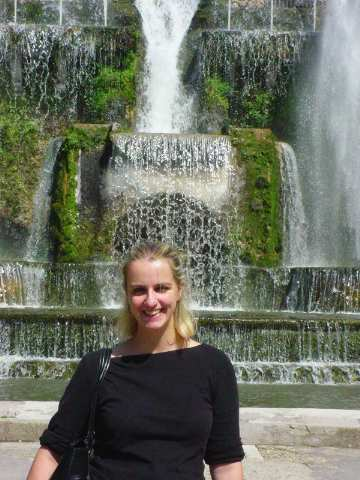
\includegraphics[width=\textwidth]{researchmicros-000.jpg}
    \caption{Original image}
  \end{subfigure}
  \hfill
  \begin{subfigure}[b]{0.49\textwidth}
    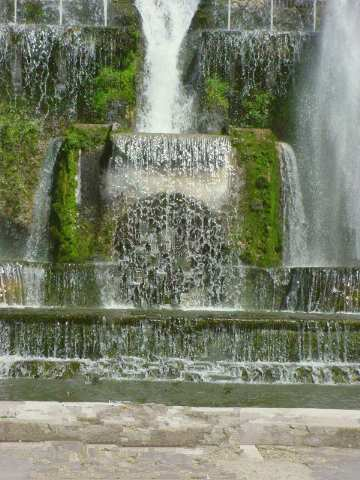
\includegraphics[width=\textwidth]{researchmicros-001.jpg}
    \caption{Object removed and gap inpainted}
  \end{subfigure}
  \label{fig:inpaint_ex}
\end{figure}

Many of the current methods are inspired by and seek to replicate the techniques used by 
professional restorators. Their underlying principle is to make use of the structure
surrounding the gap and extend it into the gap itself. Other textural details of the
surrounding are then applied.  

In particular, the literature is dominated by three classes of techniques \cite{Criminisi2004}:
\begin{description}
\item[Textural inpainting] \hfill \\
  Textural inpainting makes use of texture synthesis to fill 
  large regions with repetitive two-dimensional textural patterns.
  While these are good at replicating the textures in a consistent manner, 
  they have difficulty filling regions in photographs of real world scenes,
  which usually consist of linear or geometric structures.
\item[Structural inpainting] \hfill \\
  To address the previous issue, structural inpainting techniques specifically
  focus on propagating linear structures (called \emph{isophotes} in the literature)
  into the target region via diffusion. The method is inspired by partial differential
  equations that describes the distribution of physical heat and work well for small regions.
  For big regions, however, they introduce blur and also has the tradeoff of poorly 
  synthesizing textures. The methods proposed in \cite{Bertalmio2000,Bertalmio2001}
  belong to this this class of inpainting techniques.
\item[Combination] \hfill \\
  The method devised in \cite{Criminisi2004} combines the strengths of both approaches,
  using techniques called \emph{exemplar-based texture synthesis},
  which contains the essential process required to replicate both texture and structure.
\end{description} 

While we consider these conventional state-of-the-art methods as part of our evaluation
framework, we mostly focus on novel techniques involving multidimensional
chromatic derivatives, which can also be viewed as a combination of textural and structure
inpainting. The development and implementation of these novel techniques forms the major
portion of this thesis project. We propose our approach in \cref{proposal}. 

\newpage

%----------------------------------------------------------------------------------------
%	MAJOR SECTION 1
%----------------------------------------------------------------------------------------

\chapter{Research Proposal} \label{proposal}

\section{Approach} \label{approach} % Sub-section

Fourier analysis and other techniques traditionally used in digital signal processing
can readily be applied to image processing, since images are just signals in the spatial
domain. 

\begin{wrapfigure}{r}{0.5\textwidth}
  \vspace{-10pt}
  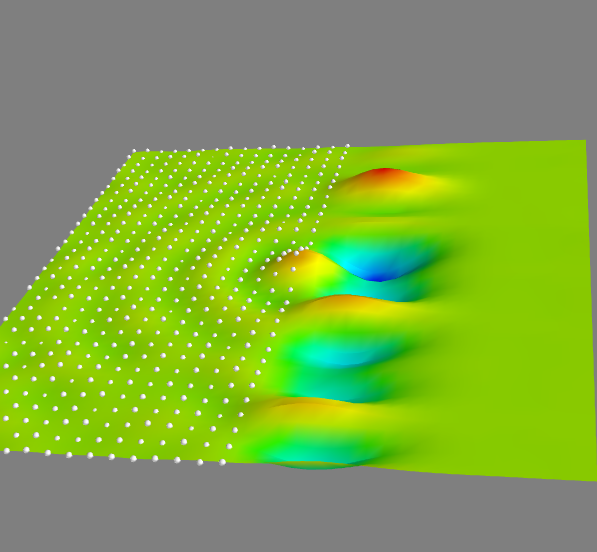
\includegraphics[width=0.48\textwidth]{31x16bump.png}
  \caption{Chromatic expansion of a signal in the spatial domain}
  \vspace{-20pt}
  \label{fig:cd_image_ex}
  \vspace{-10pt}
\end{wrapfigure}

As such, we can use the Fourier transform to decompose images into its frequency
components, or even represent an image using 2-dimensional Fourier series.

Likewise, we can represent an image using a 2-dimensional chromatic expansion,
which will be better suited for local interpolations. 
Consider \cref{fig:cd_image_ex}. Here, the white dot points are the signals
samples, while the surface is the chromatic expansion.

One thing we notice is that the surface fits the sampled points quite nicely,
creating a sort of ripple, while immediately to the right of the boundaries, 
there are some irregular peaks and valleys. We surmise that this phenomenon 
is the result of overfitting, which will be one of the first problems we have to overcome, using regularization. 

Note that at image borders, we require the texture and structure of the
border regions to extend only in an outward direction. For missing values, i.e. 
gaps within the image, we must preserve textural and structural consistency 
between all sides of the gap surroundings. For example, if a straight line 
meets a gap but obviously continues to the other side of the gap, our interpolation
must extend the line into the gap and have it join the line extending outside.

In other words, we must satisfy certain constraints imposed by the values
at the boundaries of the gap to ensure continuity across gaps.
Some work will be required to formulate this precisely as a 
mathematical programming problem in this context.

This roughly outlines the general approach and the problems we foresee at
the present time.

\section{Plan} 

Here is an outline of the plan:

\begin{enumerate}
\item Complete literature review and background readings 
  \begin{itemize}
    \item on the theory of chromatic derivatives, especially the 
    multidimensional chromatic derivatives and its expansions,
    \item state-of-the-art digital image inpainting methods
  \end{itemize}
\item Reproduce (implement) existing state-of-the-art methods
  as part of the evaluation framework for comparison
\item Develop the necessary framework for using multidimensional 
  chromatic derivatives (expansions) for image representation
\item Devise methods for inpainting based on chromatic expansions
\begin{itemize}
  \item Formalize the constraints imposed by values surrounding the gaps
  in the image, as mentioned in \cref{approach}.
  \item Develop regularization methods to prevent overfitting
\end{itemize} 
\item Implement methods above
\item Experiment with, benchmark and test the implementation empirically
\item Analyze results, revisiting 4 as needed.
\item Prepare and summarize the findings from project,
  including methods devised, implementations, results obtained, etc.
  for presentation and final thesis report.
\end{enumerate}

\chapter{Conclusion}

In this report, we gave the motivation for the chromatic derivatives
by demonstrating the shortcomings of Taylor series when processing signals.
We defined chromatic derivatives and its expansions, examined its 
properties in some detail and showed how it can be applied to image processing
problems.

In conclusion, we think chromatic derivatives are a powerful tool that promises 
many interesting and important applications. We look forward to exploring 
these applications and hope to thereby extend and further enrich the theory of
chromatic derivatives. 

%----------------------------------------------------------------------------------------
%	BIBLIOGRAPHY
%----------------------------------------------------------------------------------------

\newpage

\bibliography{../bibliography}

%----------------------------------------------------------------------------------------
%	APPENDIX
%----------------------------------------------------------------------------------------

% \appendix

% \section{Code}

%----------------------------------------------------------------------------------------
%	INDEX
%----------------------------------------------------------------------------------------

\printindex

%----------------------------------------------------------------------------------------

\end{document}